% Especificaciones del tamaño de letra, tamaño de hoja, márgenes, librerias, etc.
\documentclass[12pt, letterpaper]{article}
\usepackage[english]{babel}
\usepackage[utf8]{inputenc}
\usepackage[T1]{fontenc}
\usepackage{mathrsfs}
\usepackage{amsmath}
\usepackage{graphicx}
\usepackage{subcaption}
\usepackage{hyperref}
\usepackage{url}
\usepackage{amssymb}
\usepackage{float}
\usepackage[margin=1in]{geometry}
\renewcommand{\baselinestretch}{1.5}

% Enlace Bibliografía
\usepackage{csquotes}
\usepackage[notes,backend=biber]{biblatex-chicago}
\addbibresource{referencias.bib}

% Titulo, autores, fecha.
\title{Práctica \#5: Análisis de Perturbaciones}
\author{Carlos Vásquez 1155057}

% Inicio del documento
\begin{document}
\maketitle
\section*{Introducción}

Las perturbaciones son señales que afectan negativmente la salida de un sistema. Éstas pueden ser internas o externas. Ejemplos de perturbaciones internas puede ser el amortiguamiento que existe en un sistema o el no amortiguamiento. Para cada caso aplica una descripción distinta del sistema en cuestión, sin embargo se cuantifican y se toman en cuenta para el control de un sistema.

Existen también las perturbaciones externas, las cuales se producen fuera del sistema. Dependiendo de nuestro sistema las señales negativas pueden provenir de muchas interacciones físicas. Lo importante es que la salida que obtenemos después de que estas perturbaciones actúan no es la deseada.

Analizarlas resulta muy conveniente dado que si las entendemos podremos entender cómo eliminarlas para así obtener el resultado deseado. Un ejeplo práctico y sencillo son los \textit{auriculares con cancelación activa del ruido}. Estos auriculares pueden ser entendidos como un sistema dinámico, en el cual se está recibiendo constantemente una señal de audio. Sin embargo, las señales de audio son propensas a ruido debido al mal aislamiento de los cables y componentes electrónicos que se utilizan, al igual que el ruido que se genera en el ambiente (debido a que no existe lugar donde el nivel de sonido sea de 0 dB). Esta situación genera perturbaciones en nuestra señal de audio limpia que el consumidor desea, así que se han creado estos auriculares especiales para contrarrestar el ruido indeseable.

Los auriculares con cancelación activa del ruido utilizan las mismas propiedades del sonido para conseguir modular su señal de salida. Las ondas de sonido, al igual que otros tipos de ondas como la luz y aquellas descritas por funciones trigonométricas, son susceptibles a interferencia. Existen dos tipos de interferencia, la \textit{interferencia constructiva e interferencia destructiva}. 

\begin{figure}[H]
	\centering
	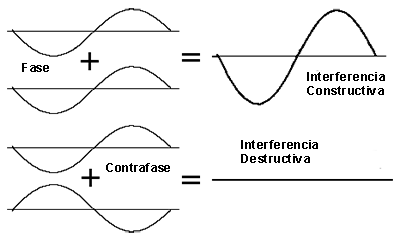
\includegraphics[width = 0.5\textwidth]{interferance.png}
	\caption{Adición de ondas, dos ondas en fase y otras desfasadas 180º.}
\end{figure}

Gracias a estas propiedades de las ondas de sonido, es posible crear un dispositivo como estos auriculares. Éstos funcionan mediante el análisis de las frecuencias que presentan ruidos innecesarios en la señal y activamente generan una señal que es polarmente opuesta al ruido de la señal original, causando interferencia destructiva y así eliminando las frecuencias innecesarias.

\begin{figure}[H]
	\centering
	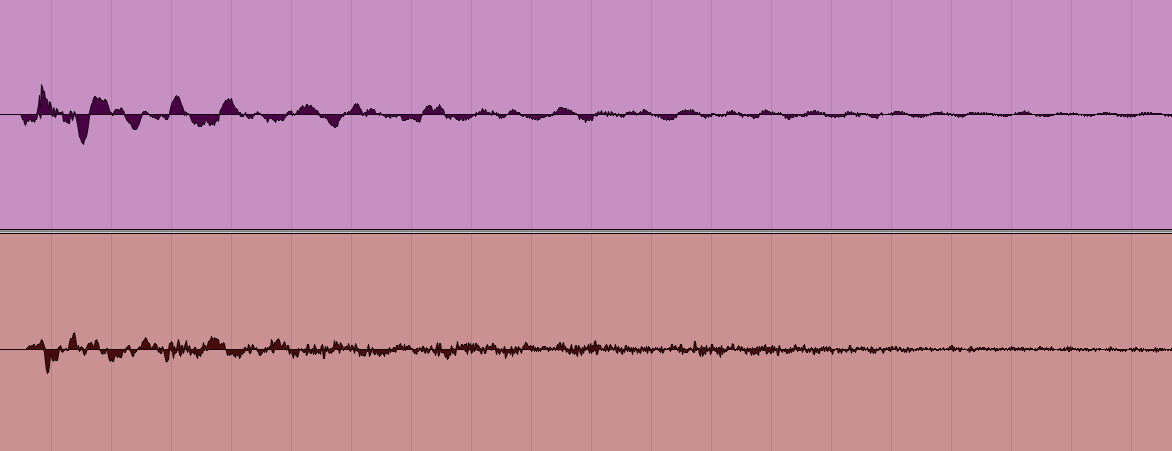
\includegraphics[width=0.7\textwidth]{noisecancel.png}
	\caption{Cancelación activa del ruido en una muestra de un tarola. Se muestra la señal original arriba y abajo la señal con la polaridad negativa encargada de cancelar frecuencias innecesarias.}
\end{figure}

\section*{Desarrollo}
\subsection*{Señal de perturbación}
Como se mostró en la sección anterior, perturbaciones pueden hacer que nuestra señal de salida no sea la apropiada y ajustar nuestro sistema ante estas perturbaciones es necesario. En esta práctica analizaremos el sistema de control implementado al modelo dinámico del péndulo hecho en una práctica anterior, sin embargo esta vez contará con una perturbación externa que afectará negativamente a nuestro sistema y, por tanto, su estabilidad a través del tiempo. Para lograr realizar una perturbación añadiremos una nueva entrada a nuestro sistema de péndulo. En este caso se decidió añadir una onda senoidal como la señal indeseada y se muestra a continuación en la figura 3.

\begin{figure}[H]
	\centering
	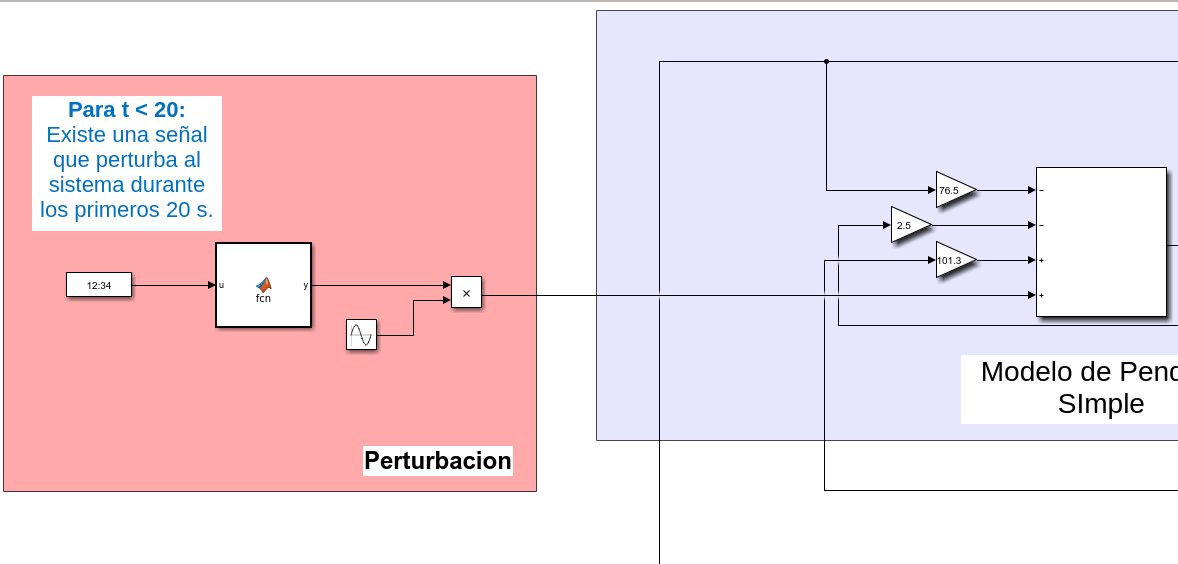
\includegraphics[width=\textwidth]{pert.png}
	\caption{Perturbación externa. Como se puede apreciar en la figura, la perturbación estará presente los primeros 20 segundos.}
\end{figure}

Para conseguir lograr esta perturbación se necesitó añadir el módulo llamado "perturbación". Éste consiste de un reloj, el cual permite medir el tiempo para registrar cuándo activarse y no activarse. También se utiliza un bloque llamado "MATLAB function" el cual permite editar y realizar una relación entre las entradas y salidas, utilizando, efectivamente, una función que nosotros definamos. En este caso, la función que hemos definido para la peturbación es análoga a la del escalón unitaro (también llamada función de Heaviside,$ \mathscr{U}(t)$).

El funcionamiento de la función que se encarga de la perturbación se muestra en la siguiente figura.

\begin{figure}[H]
	\centering
	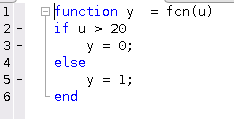
\includegraphics[width=0.6\textwidth]{pertfunc.png}
	\caption{Nuestra función consiera la entrada (u), que en este caso es el reloj que colocamos al inicio y espera hasta que el tiempo asciende a los 20 segundos para modificar su salida de 1 a 0.}
\end{figure}

Sin embargo lo que deseamos es una señal senoidal, no una constante, por lo que la salida de esta función estará siendo multiplicada por una onda senoidal con frecuencia y amplitud conocida. Esto para así activar la señal de perturbación en el tiempo que es deseado. Esto es fácil de apreciar en la figura 3.
\subsection*{Ganancias dinámicas}
Ver cómo la señal de perturbación se activa y desactiva en nuestro sistema es muy predecible, sin embargo podemos modificar las ganancias de nuestro controlador para así poder visualizar la efectividad de los distintos dieños del controlador.

En la práctica anterior se exploró el concepto de las sumas ponderadas y cómo éstas afectan el la influencia que cada error tiene sobre el sistema en general. Si las ganancias de nuestro sistema son estáticas simplemente veremos la señal cuando la perturbación entra en nuestro sistema y cuando desaparece obtendremos el mismo sistema dinámico de la práctica anterior.

\begin{figure}[H]
	\centering
	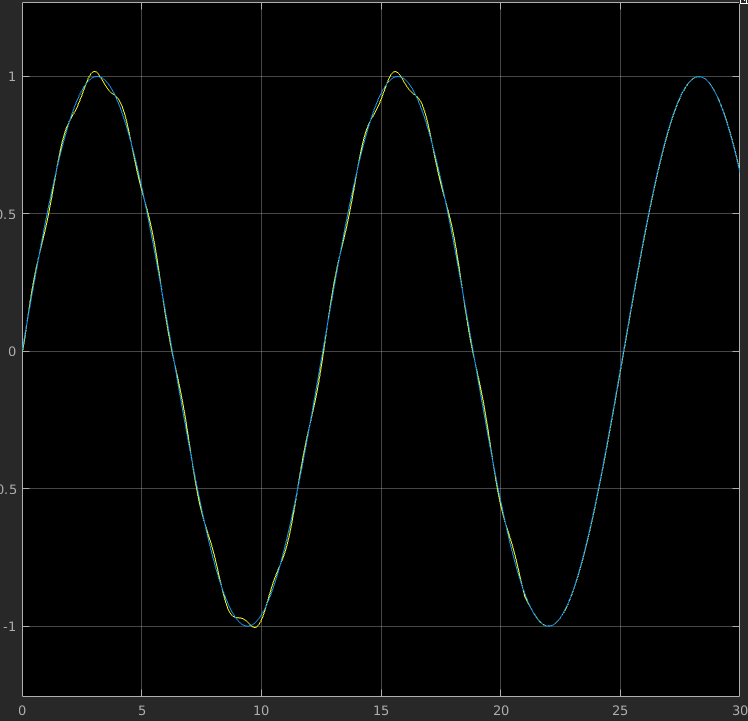
\includegraphics[width=0.6\textwidth]{sgain.png}
	\caption{Se aprecia la perturbación los primeros 20 segundos, después el sistema es el mismo que el original.}
\end{figure}

Sin embargo, si queremos entender más cómo afectan las distintas ganancias al sistema dinámico, entonces podemos generar algo parecido a lo que realizamos con la perturbación, pero con la ganancias. En este caso, el valor de las ganancias serán determinados por el tiempo. De 0 a 10 segundos las ganancias serán las originales, donde $a_1 = 90$ y $a_2 = 10$. De 10 segundos en adelante las ganancias cabiarán, donde $a_1 = 200$ y $a_2 = 30$.

\begin{figure}[H]
	\centering
	\begin{subfigure}[b]{0.49\linewidth}
		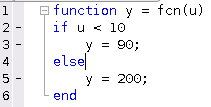
\includegraphics[width=\linewidth]{a1.png}
		\caption{Función para $a_1$}
	\end{subfigure}
	\begin{subfigure}[b]{0.49\linewidth}
		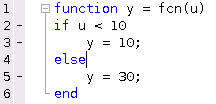
\includegraphics[width=\linewidth]{a2.png}
		\caption{Función para $a_2$}
	\end{subfigure}
	\caption{Ganancias dinámicas definidas.}
\end{figure}

En diagrama de bloque nuestras ganacias dinámicas se muestran como el siguiente módulo:

\begin{figure}[H]
	\centering
	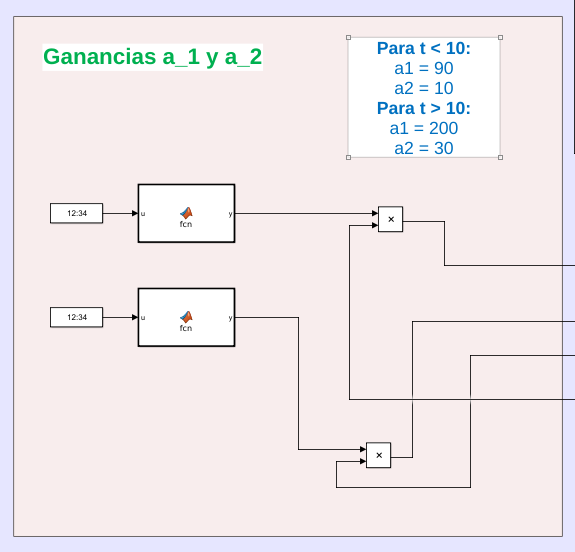
\includegraphics[width=0.7\textwidth]{dgain.png}
	\caption{Se muestra el diagrama de bloque para estas funciones. La multiplicación se lleva a cabo con los errores de la ecuación diferencial descrita en la práctica pasada.}
\end{figure}

Estas ganancias dinámicas afectarán a través del tiempo a nuestro sistema, ésto lo podemos ver reflejado en la siguiente gráfica que muestra la posición ideal y la posición real con la señal de perturbación y las ganancias dinámicas implementadas.

Estos cambios son los únicos que deseábamos añadir, por lo que el sistema de control está completo. En la figura 9 se muestra el sistema de control en forma de diagrama de bloque.

\begin{figure}[H]
	\centering
	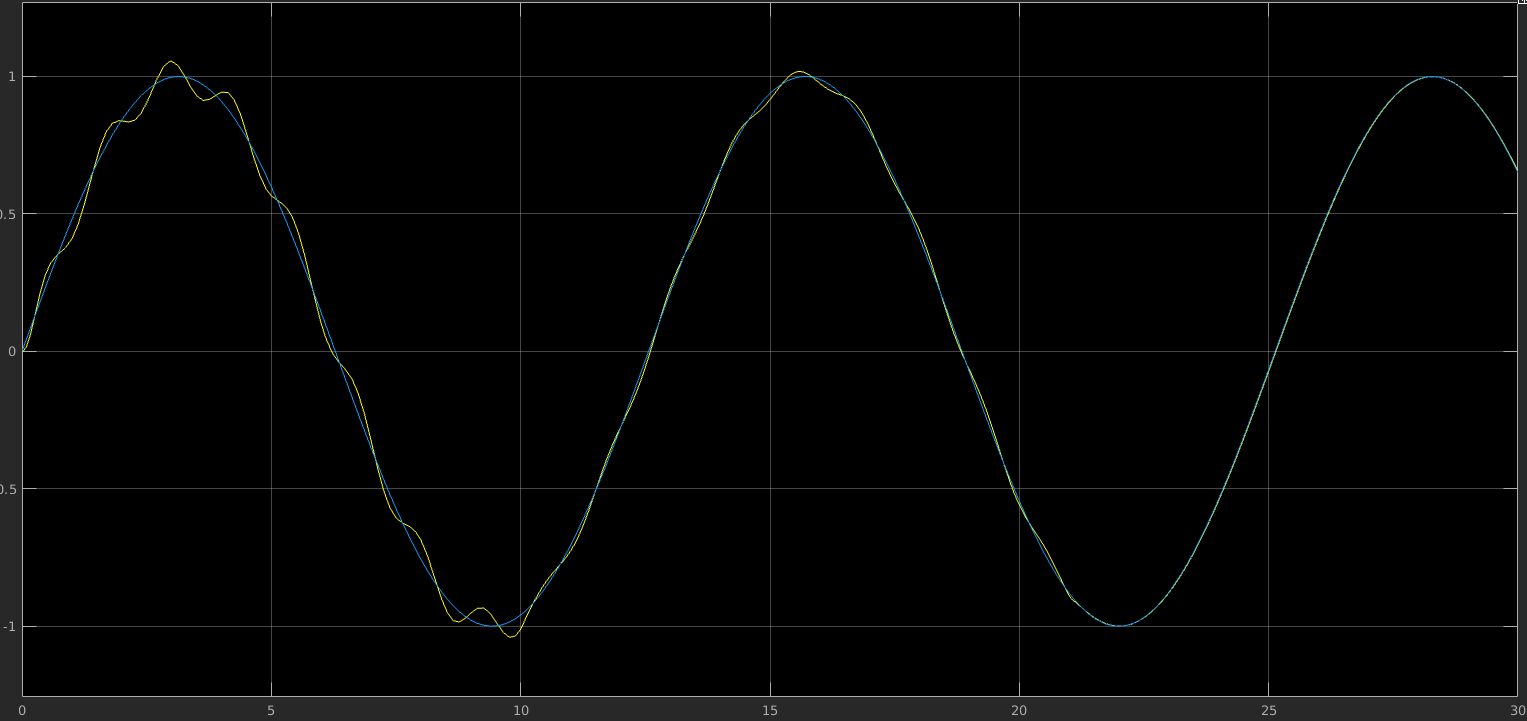
\includegraphics[width=0.9\textwidth]{fullsys.png}
	\caption{Se puede observar cómo cambia el sistema a través del tiempo y cuándo las ganancias cambian de valor en $t = 10 s$. También se observa cuando la perturbación cesa en $t = 20 s$}
\end{figure}


\begin{figure}[H]
	\centering
	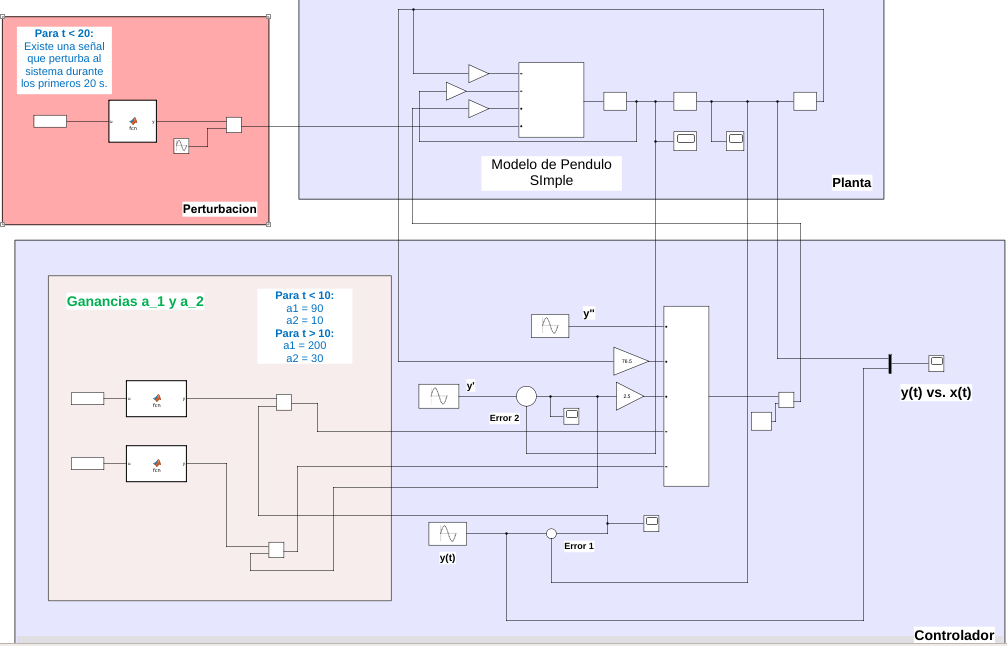
\includegraphics[width=\textwidth]{blockfull.png}
	\caption{Sistema de control completo, aunado a una perturbación.}
\end{figure}

\section*{Conclusión}

A partir del ejemplo de la introducción sobre los auriculares que cancelan el ruido en sus señales, es muy claro que la comprensión de las perturbaciones coo señales es de gran importancia. Esto es fácil de apreciar en el sistema del péndulo, debido a la nueva señal de entrada nuestro sistema se volvió inestable. Si lo que deseamos es minimizar el error con la referencia, entonces estas perturbaciones vuelven estos errores muy grandes, lo cual es peligroso si hablamos de sistemas más complicados como aeronaves o biocontroladores. Es por esto que minimizar estos errores y optimizar nuestros sistemas es de tanta importancia.

\begin{figure}[H]
	\centering
	\begin{subfigure}[b]{0.49\linewidth}
		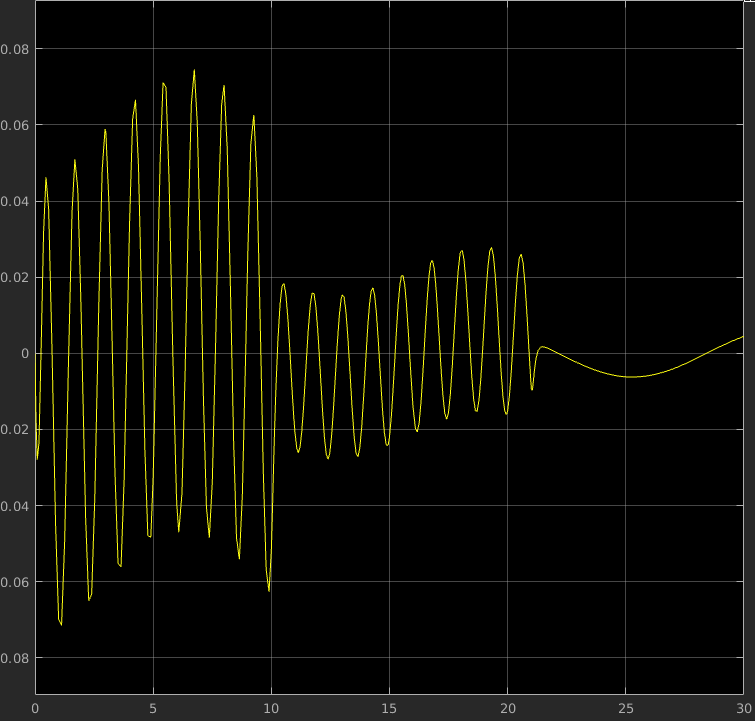
\includegraphics[width=\linewidth]{e1.png}
		\caption{Magnitud de $e_1$}
	\end{subfigure}
	\begin{subfigure}[b]{0.49\linewidth}
		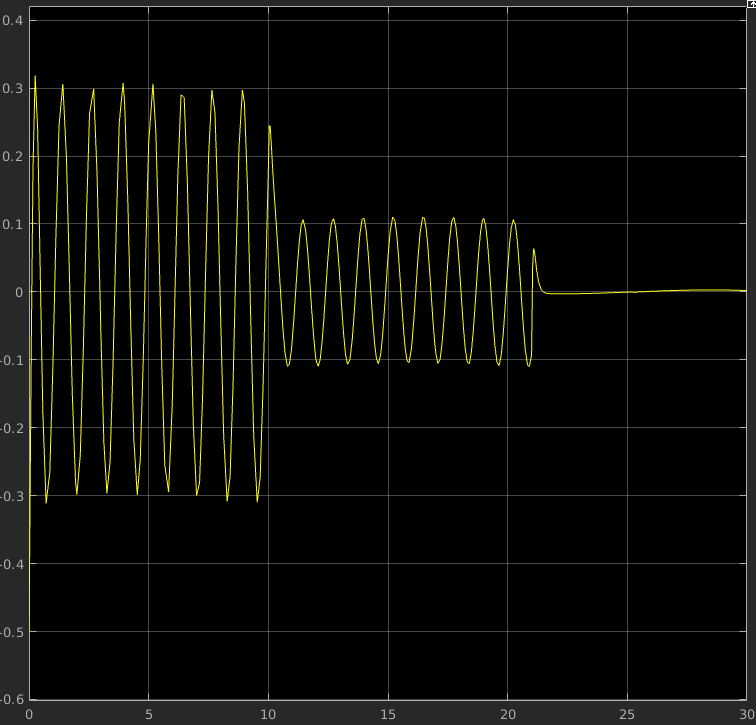
\includegraphics[width=\linewidth]{e2.png}
		\caption{Magnitud de $e_2$}
	\end{subfigure}
	\caption{Cambio en los errores cuando la perturbación y las ganancias dinámicas están en el sistema. Es posible apreciar la gran diferencia en los errores con los que se contaba en la práctica pasada a comparación de los mostrados en la figura.}
\end{figure}

%%%%%  Bib
\renewcommand\refname{Referencias}
\printbibliography
\end{document}
